
\section{Dual Processes in Reasoning}
\label{sec:chapter1-dual-process}

From \citet{Wason1975} onwards,
reasoning researchers have considered the possibility
that responses on reasoning problems can be generated by one of two
qualitatively different kind of process.
Versions of this distinction have been proposed
many times in many different fields,
leading to considerable confusion as to
what defines each kind of process
\citep[see][]{Evans2013a,Stanovich2012,Evans2008}.
Proposed distinctions include those between \citep[from][]{Evans2008}
input modules and higher cognition \citep{Fodor1983},
automatic and controlled processes \citep{Schneider1977},
heuristic and analytic processes \citep{Evans1984,Evans2006},
and associative and rule-based systems \citep{Sloman1996},
among many others.
More recent accounts \citep[e.g.][]{Evans2013a}
offer a distinction that somewhat simplifies the matter:
Type 1 processes are a heterogeneous set of processes,
some, but not all, of which are dependent on specific neural subsystems,
which operate automatically in the presence of their enabling conditions
\citep[that is, they are \emph{autonomous};][]{Stanovich2009},
and do not require conscious effort.
Type 2 processes, in contrast, are mental operations that require
a) the formation, manipulation, and updating of
an abstract representation in working memory, and
b) the \emph{decoupling} of this representation from Type 1 processes
\citep[see][]{Stanovich2012}.
This account can be further simplified 
without much loss in the central message:
Type 2 processes are those which require working memory,
while Type 1 processes are those that do not.

It should be noted, however, that
dual process accounts are not without controversy.
There has been extensive criticism of such accounts
both in the reasoning literature
\citep{Kruglanski2013,Kruglanski2011,Gigerenzer1996a,Osman2004}
and more generally \citep[e.g.][]{Newell2014,Tunney2003}.
In particular, \citet[][also \citealp{Gigerenzer1996a}]{Kruglanski2011}
argue that Type 1 and Type 2 processes
both reflect the application of cognitive rules,
and that these rules differ only quantitatively
in how much mental effect they require,
and how consciously accessible they are.


\subsection{Conflict in Dual Process Theories}
\label{subsec:chapter1-dual-process-conflict}

My interest in dual process theories in this thesis
centres on their potential to explain conflict during reasoning.
How and when this conflict occurs depends
on how Type 1 and 2 processes interact.
A common thread throughout dual processes accounts
is that Type 1 processes in many contexts
produce responses that are heuristic, biased, and inappropriate,
whereas Type 2 processes, when used,
typically lead to normatively correct responses.
In this sense, dual process theories build on
the earlier Heuristics and Biases research tradition
\citep{Gilovich2002,Tversky1974,Kahneman1982}.
This tradition focused on situations where
people often rely on mental shortcuts, or \emph{heuristics}
instead of engaging in more effortful decision making,
leading to systematic biases in situations where
the heuristic does not provide a useful solution
to the problem at hand.
More recent treatments of the heuristics and biases literature
\citep{Kahneman2005,Kahneman2002,Kahneman2011}
have explicitly described heuristics as the result of Type 1 processes,
while the \emph{reflective} thinking
needed to resist these heuristic responses \citep{Frederick2005}
is the consequence of Type 2 processes
\citep[although, again, see][for contrasting views]{Gigerenzer2011,Kruglanski2011}.

\citeauthor{Evans2007a} (\citeyear{Evans2007a}; \citealp[see also][]{Gilbert1999})
argues that there are three possible ways in which
Type 1 and Type 2 processes could interact.
He labels these
\emph{pre-emptive conflict resolution},
\emph{default-interventionist},
and \emph{parallel-competitive} architectures
\citep[perhaps more intuitively referred to as
  \emph{selective}, \emph{corrective}, and \emph{competitive} designs by][]{Gilbert1999}.

Simplest are selective, pre-emptive conflict resolution models
\citep{Chaiken1987, Petty1986, Klaczynski2000, Klaczynski2004},
where a given decision cues the activation of
either Type 1 \emph{or} Type 2 processes.
Clearly, there is little role for conflict in such accounts,
as only one or other kind of process should be active at any one time.
\citet{Gilbert1999} notes that such models are popular
with researchers interested in predicting overt behaviour
rather than inferring underlying processes,
and so have proven resilient within social psychology,
often as models of persuasion
\citep{Petty1986,Chaiken1987}.
Klaczynski \citetext{\citeyear{Klaczynski2000}; \citealp{Klaczynski2004}}
proposes an analogous model in the reasoning literature.
Although they do not account for conflict during reasoning,
selective dual process models provide
a parsimonious account of participants' responses on many tasks.
In early dual process research, it was these responses that were the focus of analysis:
researchers primarily analysed only the choices participants made,
such as numerical judgements \citep[e.g.][]{Tversky1981},
ratings of the persuasiveness of arguments \citep[e.g.][]{Chaiken1987},
or judgements of validity of logical syllogisms \citep[e.g.][]{Evans1983}.
Many theories that initially proposed selective activation,
however, have subsequently been updated to account for
results that suggest conflict or interference,
and so have developed into default-interventionist
or parallel-competitive accounts.
\citet{Evans2007a} highlights an additional limitation of these models:
they require, but often fail to provide, some means of deciding which process should be engaged.


Corrective, default-interventionist models
\citep{Evans2006, Kahneman2005,Kahneman2002}
provide an alternative account.
According to these models
--- typically the best known in the literature,
particularly following the publication of \citegap{Kahneman2011}{'s}
\emph{Thinking, Fast and Slow} ---
Type 1 processes are constantly active,
cuing responses, generating mental representations, and processing incoming stimuli.
The main role of Type 2 processes is to 
monitor and inspect these intuitive beliefs and responses,
and to inhibit or override them if they are found to be inadequate.
If the output of a Type 1 process is deemed inappropriate,
it must be inhibited, and possibly replaced
with the product of more effortful Type 2 thinking.
Most theories hold this monitoring processes is typically lax
--- people are \emph{cognitive misers} \citep{Fiske1991} ---
and so under most circumstances we give intuitively-produced responses
and engage in intuitively-cued behaviours
\citep{Tversky1974, Tversky1973, Kahneman1982, Kahneman1973,
  Kahneman2005, Kahneman2002, Stanovich1999, Gilovich2002}.
Conflict, however, occurs when people detect that
their intuitive responses are inadequate,
and attempt to inhibit or override them.

In competitive, or parallel-competitive models \citep{Sloman1996,Sloman2014a,Sloman2014,Darlow2010,Sloman2002},
both Type 1 and Type 2 processes are thought to be activated simultaneously.
An important aspect of \citegap{Sloman1996}{'s} model,
although also consistent with default-interventionist accounts,
is that parallel activation of both kinds of process would allow
people to simultaneously hold two potentially contradictory beliefs,
one generated by each kind of process \citep[Criterion S;][]{Sloman1996}.
Parallel models differ from their interventionist counterparts
in that they would predict conflict to be much more common in cognition.
If both Type 1 and Type 2 processes are activated during reasoning,
then both may simultaneously cue conflicting responses.
When this happens, participants should be conflicted
regardless of what response they actually give ---
they will be partially drawn to the Type 1 response
if giving the Type 2 one, and vice versa.

Although not included in \citegap{Evans2007a}{'} review,
more recent accounts,
while still operating within a dual process framework,
have questioned the notion that
Type 1 processes are always biased,
and that Type 2 processes are essential for sound reasoning.
First, a number of experiments
\citep[e.g.][]{DeNeys2008,DeNeys2008a,DeNeys2011b,DeNeys2013a,
  DeNeys2010,DeNeys2008a,Morsanyi2012}
have compared problems where
participants predominantly give the incorrect, heuristic response
to no-conflict versions where
the heuristic response is the correct one.
In these experiments, participants rarely
explicitly report that they realise their heuristic responses
are suspect \citep{DeNeys2008}.
However, using more subtle implicit measures,
these experiments have shown that participants
are sensitive to the conflict between
their heuristic responses and normative principles;
for instance, on conflict trials participants
are slower to respond \citep{DeNeys2008a},
are less confident in their responses \citep{DeNeys2011b, DeNeys2013a},
sweat more \citep{DeNeys2010},
show greater activation in the anterior cingulate cortex,
a neural region implicated in the detection of conflict \citep{DeNeys2008a},
and even report ``liking'' logically valid syllogisms
more than equivalent invalid ones \citep{Morsanyi2012}.
For clarity, I will refer to De Neys' \citep[e.g.][]{DeNeys2008} proposal
that reasoners who give heuristic responses
detect some conflict while doing so
as the \emph{dual process conflict monitoring theory}.
This accounts draws on theories of conflict monitoring
in simpler cognitive domains \citep{Botvinick2001}.

More recent work \citep[i.e.][]{DeNeys2012, DeNeys2014a}
proposes a stronger interpretation of these results:
that Type 1 processes can simultaneously cue
both the sometimes incorrect heuristic response
and the logically correct response.
Clearly, this is a stronger claim than that made by
the dual process conflict monitoring theory,
and I will reserve the name \emph{intuitive logic} theory for this account.
According to this stronger account,
participants predominantly give the heuristic response
because it is cued more strongly by Type 1 processes
than the correct one (i.e. it is \emph{prepotent}).
Type 2 processes, in this account, are activated when
participants detect a conflict between
multiple responses generated by Type 1 processes,
and must inhibit the prepotent heuristic response
in order for participants' to produce the correct response.
However, according to \citet{DeNeys2013},
while participants will usually detect this conflict,
and attempt to engage Type 2 processes,
they often fail to inhibit the heuristic response,
leading to biased reasoning.
A similar account is offered by \citet{Handley2015},
who in addition to arguing that Type 1 processes
can produce both heuristic and correct responses,
claim that Type 2 processes can also be responsible
for the generation of biased responses.
Finally, \citet{Pennycook2015} offer a framework
that formalises the interaction of multiple Type 1 responses
proposed by \citet{DeNeys2012,DeNeys2014a}.
For the purposes of this thesis,
the differences between these theories are not particularly germane.
Therefore, I will restrict my discussion for the most part
to the intuitive logic theory \citep{DeNeys2012,DeNeys2014a},
with the understanding that points applicable to it
are also relevant to the accounts put forward by \citet{Handley2015}
and \citet{Pennycook2015}.


Intuitive logic theories,
like parallel-competitive accounts,
predict that conflict should be common in reasoning.
Both of these  accounts predict that
participants should experience conflict
even when they give a heuristic response.
The intuitive logic account holds that this happens because
both responses are cued by Type 1 processes,
and the role of Type 2 processes is to
select between candidate responses,
and to engage and direct the inhibitory processes
needed to hold back the prepotent heuristic response.
The parallel-competitive account, on the other hand, holds that
Type 2 processes cue the logical response
at the same time as Type 1 processes cue the heuristic one.

\begin{table}
  \centering
  \caption[Predictions about conflict from various dual process theories]{
    When do different dual process theories predict that conflict should occur?
    \emph{Note:} T1 = Type 1 processes; T2 = Type 2 processes.
  }
  \begin{tabular}{l L{.3\textwidth} L{.3\textwidth} }
    \toprule
    & T1 responses                & T2 responses \\ %
    \midrule
    %% \endhead
    Selective               & No                          & No \\
    Default-Interventionist & No                          & Yes (inhibit~T1~response) \\
    Parallel-Competitive    & Yes (T2~interference)       & Yes (T1~interference) \\
    Intuitive logic         & Yes (multiple~T1~responses) & Yes (inhibiting~prepotent~T1~response) \\ 
    \bottomrule 
  \end{tabular}
\end{table}


\subsection{Factors dictating the generation of Type 1/Type 2 responses}
\label{subsec:chapter1-dual-process-factors}


So far, I have discussed the circumstances under which
various dual process theories would predict that conflict should occur.
However, one important question remains:
in situations where these processes do conflict,
how is this conflict resolved?
In this section, I introduce a number of recent frameworks proposed
to make sense of why people sometimes
produce responses, generated by Type 1 processes,
and other times correct responses, generated by Type 2 processes
\citep[but again, see][]{DeNeys2012, Handley2015}.

\citet{Stanovich2008} provide one such framework,
in their discussion of individual differences
in susceptibility to various heuristics and biases,
which is equally applicable to the question of conflict in reasoning.
Their framework is based on default-interventionist dual process accounts,
where the heuristic, Type 1 response is given
unless overridden by Type 2 processes.
Firstly, if participants do not know
the logical rules required to produce the correct response
\citep[the \emph{Mindware}, in the terms of ][]{Stanovich2008},
they will not be able to do so.
After this, participants must realise that
their heuristic response is inadequate,
something which some theories \citep{DeNeys2012} hold to happen automatically,
while others \citep{Evans2006,Evans2013a,Kahneman2011} believe
this requires motivated attention
and the engagement of Type 2 processes.
Thirdly, some tasks require executive processes
to inhibit the heuristic response,
and to form and manipulate the necessary
\emph{decoupled} representation in working memory
in order to reach the logically valid response.
On tasks for which this is not necessary,
it should be trivially easy for participants who
understand the logical principles, and realise their intuitions are mistaken,
to produce the logical response.
Where it is necessary, however, participants must
engage these executive processes in order to respond correctly,
and so it is at this point where conflict should occur.
Figure~\ref{fig:stanovich} shows a schematic of this framework.

\begin{figure}[ht]
  \centering
  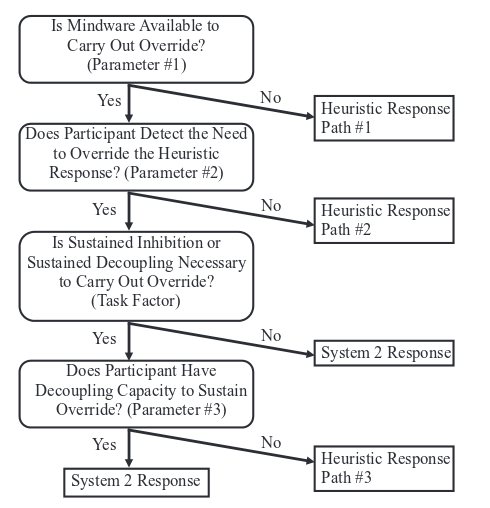
\includegraphics[width=.5\textwidth]{imgs/stanovich.png}
  \caption[The \citet{Stanovich2008} framework for individual differences in reasoning.]{
    \protect{\citegap{Stanovich2008}{'s}} framework for individual differences in reasoning.
    From \protect{\citet{Stanovich2008}}.
  }.
  \label{fig:stanovich}
\end{figure}



\citet{DeNeys2013} discuss a similar issue, and highlight
three possible ``failures'' that lead participants to give incorrect, heuristic responses.
Their \emph{storage} failure is analogous to \citegap{Stanovich2008}{'s} Mindware gap:
participants who do not possess the knowledge necessary to respond correctly
--- the rules of formal logic, or probability theory, for instance ---
will respond heuristically.
Their \emph{monitoring} failure occurs when participants,
although possessing the correct knowledge,
fail to realise that their heuristic responses are inconsistent with that knowledge.
Finally, their \emph{inhibition} failure occurs when
participants do detect the inadequacy of their heuristic response,
but fail to properly inhibit it.

\citet{DeNeys2013} also draw attention to the issue of
\emph{when} individual differences between
heuristic and rational reasoners should emerge.
Differences due to storage failures should emerge
at the very onset of reasoning:
participants without the correct knowledge will be biased from the start;
those with that knowledge will reason correctly .
Such a failure may be analogous to a selective dual process account
\citep{Klaczynski2004}.
Differences due to monitoring failures should emerge slightly later,
as some participants realise that their heuristic responses,
once generated, are incorrect, while others do not.
This corresponds to the classical default-interventionist account \citep{Evans2006}.
Lastly, differences due to inhibition failures
should emerge latest of all:
participants realise that their heuristic responses are inadequate,
and attempt to inhibit them, but only some manage to complete this inhibition.
This possibility accords most closely with the intuitive logic account \citep{DeNeys2012}.



Finally, \citet{Pennycook2015} put forward a dual process framework
that consolidates aspects of default-interventionist dual process accounts \citep[e.g.][]{Evans2006}
and the intuitive logic theory \citep{DeNeys2012}.
This framework is illustrated in Figure~\ref{fig:pennycook}.
In line with the intuitive logic theory,
they propose that, when faced with a problem or cue,
Type 1 processes can generate multiple responses,
often including the correct one.
If participants fail to detect a conflict between these multiple responses
(or, presumably, if they only generate one response),
then they will give the prepotent, or heuristic response,
which is incorrect in many tasks studied in the lab.
If they do detect a conflict, participants activate Type 2 processes.
With these, they can either a) engage in \emph{rationalisation},
attempting to justify the heuristic response already cued by Type 1 processes,
b) inhibit this prepotent response and give one
of the other intuitively-produced responses, or
c) inhibit the prepotent response and explicitly work out a new response,
not cued by Type 1 processes.

\begin{figure}[ht]
  \centering
  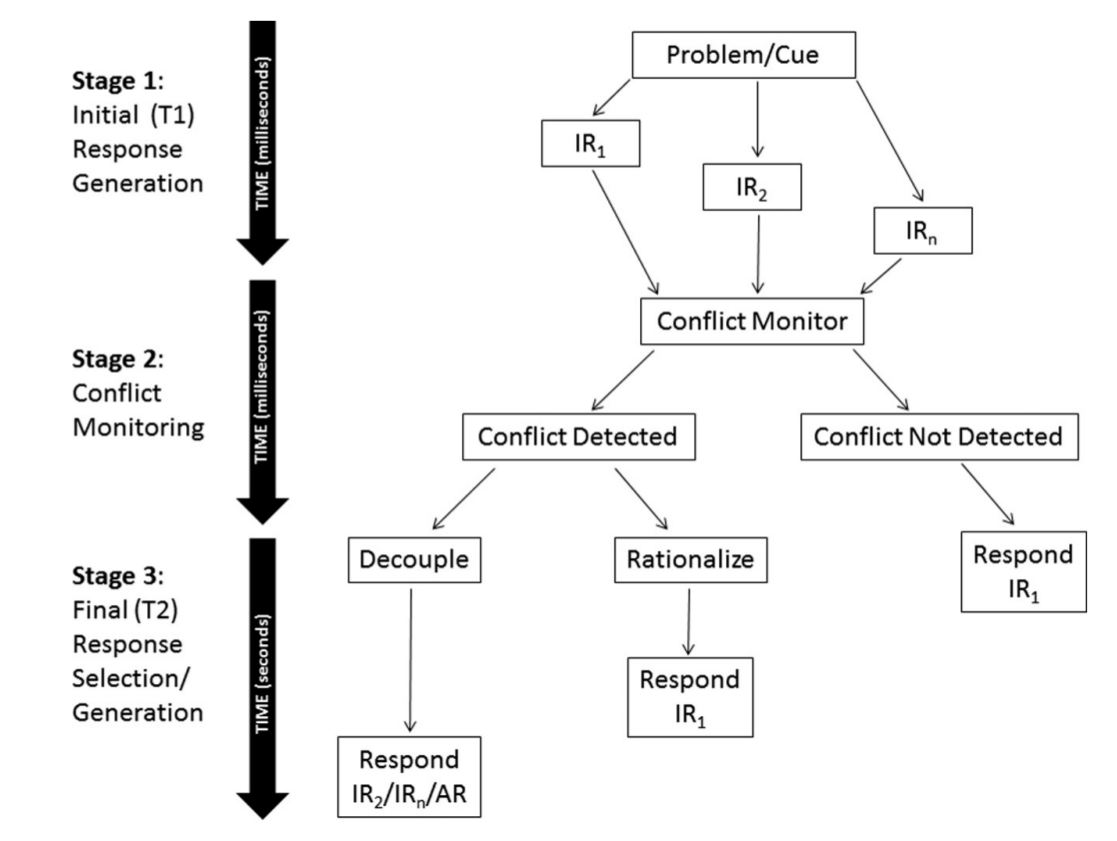
\includegraphics[width=.7\textwidth]{imgs/pennycook.png}
  \caption[The dual process framework proposed by \citet{Pennycook2015}.]{
    The dual process framework proposed by \citet{Pennycook2015}.
    From top to bottom: once participants are presented with a cue,
    they generate a number of intuitive responses ($IR_1$,  $IR_2$, $IR_n$)
    in parallel, using Type 1 processes.
    If they do not detect conflict between these responses,
    they will proceed to give the prepotent response, $IR_1$.
    If they do detect a conflict,
    they will attempt to engage Type 2 processes,
    and either seek to justify their strongest intuitive response $IR_1$
    (that is, they \emph{rationalise} it),
    or inhibit $IR_1$ in favour of one of the other intuitive responses,
    or alternatively reach a new response ($AR$)
    through Type 2 reasoning.
    From \citet{Pennycook2015}.
    \label{fig:pennycook}
  }
\end{figure}

From the above, it is clear that
conflict has come to play an important role
in dual process theories of reasoning.
Later in this thesis, I present experiments
where I use the mouse tracking paradigm
to reveal more about conflict between
Type 1 and Type 2 processes.
If we are to study this conflict, however,
we need a means of investigating it empirically in the lab.
In the next section,
I discuss how this can be achieved in general,
and in particular how I achieve it in this thesis.

